\documentclass{article}
\usepackage[spanish]{babel}
\usepackage{graphicx}
\usepackage[utf8]{inputenc}
\usepackage[spanish]{babel}
\usepackage{natbib}
\usepackage{float}
\usepackage{amsmath}
\usepackage{amssymb}
\usepackage{array}

\usepackage{tikz}
\usetikzlibrary{shapes.geometric, arrows}

\tikzstyle{startstop} = [rectangle, rounded corners, minimum width=3cm, minimum height=1cm,text centered, draw=black, fill=red!30]
\tikzstyle{process} = [rectangle, minimum width=3cm, minimum height=1cm, text centered, draw=black, fill=orange!30]
\tikzstyle{decision} = [diamond, minimum width=1.5cm, minimum height=0.8cm, text centered, draw=black, fill=green!30,font=\footnotesize]
\tikzstyle{arrow} = [thick,->,>=stealth]


\title{Clasificación inteligente sinergia entre lógica difusa y algoritmos genéticos }
\author{José Adrián Rodríguez González}
\date{Octubre 2024}
\begin{document}
\maketitle
\section{Introducción}
Para el mes de octubre se leyó la literatura acerca de los algoritmos genéticos y la lógica difusa propuesto por \citep{article1}, en este primer articulo menciona varios aspectos importantes de implementación de estos métodos. A su vez que en \citep{413232}, explica otra metodología de aplicación para crear seleccionar reglas difusas.
\section{Métodos de selección de sistemas difusos.} 
\subsection{Método Michigan.}
Primeramente, se crea un conjunto difuso \(A\) que contiene \(n\) subconjuntos difusos, que dependerán de \(x_i\) caracterísitcas de un conjunto de datos, siendo 
\[ A=\{A_i |A_i \subseteq A\} \wedge A_i=\{(x_i,\mu(x_i))|x_i \in X\}\]
Los subconjuntos difusos se puede definir como (tabla \ref{table:Table1}):
\begin{figure}[h]
    \centering    
    \begin{tabular}{|c|c|}
        \hline
        Nivel & Valor \\ \hline
        Very Low & 1 \\
        \hline
        Low & 2 \\
        \hline
        Medium & 3 \\
        \hline
        High & 4 \\
        \hline
        Very High & 5 \\
        \hline
    \end{tabular}
    \caption{Tabla de conjuntos difusos enumerados}
    \label{table:Table1}
\end{figure}
    

Después, se debe de tener un vector \(V\), cada indice \(i\) del vector es una característica \(x\) del conjunto de datos, y los elementos del vector son un conjunto difuso \(A_i\).

\[ v_1 =[2,1,3,5]   \]
Esto significa, que los valores 2,1,3 y 5 son subconjuntos difusos de \(A\),y  la posición 0,1,2,3 son las características, por lo tanto, a la característica 0 se le evalúa con el segundo subconjunto difuso, la característica 1, es el primer subconjunto difuso, y de esa forma, se pueden definir reglas, tales como
\begin{equation*}
    \begin{split}
        \text{ if } x_1 \text{is low and }  x_2 \text{is very low and } x_4 \text{is medium and } x_5 \text{is very high } \\
        \text{then is Class 1 with CF:} 0.83
    \end{split}
\end{equation*}
El \(CF\) es el grado de confianza de que sí es la clase dicha, para ello, se deben de realizar los siguientes cálculos:


Se calcula \[\beta_{CT}=\sum_{x_{p1}\in CT} \mu_i^K(x_{pq})*\mu_j^K(x_{p2})\], De forma generalizada,ya que esta manera de expresarlo es en base a dos características.
\[\beta_{CT}=\sum_{x_{p1}\in CT} \prod_{q=0}^{Q}\mu_i^K(x_{pq})\]
Siendo \(q\) uns característica y \(Q\) el conjunto de características que \(q\subseteq X_q\).
Se Multiplica cada una de las funciones de activación dadas por la regla de todas las características seleccionadas de cada instancia del conjunto de datos. \(CT\) es una clase especifica, por lo que debemos de separar nuestro conjunto de datos por las clases que existan, de esa manera, la sumatoria de las multiplicaciones de los subconjuntos difusos de cada característica será el \(\beta_{CT}\) de esa clase.
Si un \(\beta_{CT}=0\), eso significa que esa regla es incompatible para esa clase.

Al conjunto de \(\beta_{CT}\), se busca aquel que tenga el máximo valor, de tal manera que:
\[\beta_{CX}=\max\{\beta_{C1},\beta_{C1},\dots,\beta_{CM}\}\]
Si dos o más clases tienen el mismo valor o todos valen 0, entonces \(C^k_{ij}\) no puede ser determinado, por lo que este tipo de reglas se les considera \textit{dummies}, se les suele llamar como \(\phi\), sino \(C^k_{ij}=CX\)
Ya que se pudo generar esa clase, entonce se calcula el grado de confianza de esa clase.
\[CF^K_{ij}=\frac{(\beta_{CX}-\beta)}{\sum_{T=1}^{M}\beta_{CT}}\]
Donde \[\beta=\frac{\sum_{T=1,T\neq X}^{M}\beta_{CT}}{(M-1)}\]
De esa forma, podemos encontrar la tasa de confianza que posee una regla dada a una clasificación.

Para poder clasificar un patrón, o instancia,se generar un \(S\) conjunto de reglas, siendo \(R_{ij} \subseteq S\), después, se calcula  el \(\beta_{CT}*CF^K_{ij}\) de la instancia \(x_p\), para todas las \(R_{ij}  \subseteq S\), de tal forma, que se encuentra el valor máximo de este calculo de todo el conjunto de reglas y la clase asociada a la regla, será la clasificación del patrón.
\[\alpha_{CT}=\max\{\prod_{q=0}^{Q}\mu^K_{i}(x_{pq})*CF^k_{i}|C^k_{i}=CT,R^k_i \in S\}\]
De esta forma el\(X(CX)\) es 
\[\alpha_{CX}=\max\{\alpha_{C1},\alpha_{C2},\alpha_{C3},\dots,\alpha_{CM}\}\].

\subsection*{Selección}
La selección para este modelo de acuerdo a lo propuesto por \citep{article1},se hace una ruleta de probabilidades.
\begin{equation*}
    P(R_j)=\frac{f(R_j)-f_{min}(S)}{\sum_{R_i\in S}\{f(R_j)-f_{min}(S)\}}
\end{equation*}
\subsection*{Cruza y mutación}
Acorde a (Fig.\ref{fig:fig1}), la mutación es una cruza de los cromosomas de los individuos seleccionados, y la mutación es un ligero cambio que se realiza en el gen de un individuo.
\begin{figure}[h]
    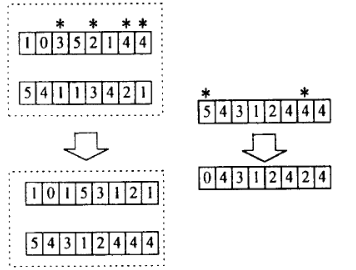
\includegraphics[width=0.5\textwidth]{image1.png}
    \caption{Cruza y mutación}
    \label{fig:fig1}
\end{figure}
La pieza clave para Michigan, es que el algoritmo genético se emplea a cada regla del conjunto.
\subsection{Método Pittsburgh.}
Pittsburgh emplea el mismo proceso, solamente, que en vez de realizarlo en base a reglas individuales, lo hace por subconjuntos de reglas, de tal manera que tanto las formulas de evaluación, como de selección, se hace en base a un conjunto de reglas

Para escoger el método, dependerá del tipo de problema que estemos manejando, no siempre se usan los mismo métodos para todos los problemas, ya que en algunas ocasiones, no resultan en un sistema óptimo.

\section{Trabajo del mes}
Como se puede observar, se recopilo la información de Ishibuchi, sin embargo, también se realizó un primer modelo en un problema de clasificación binaria como el conjunto de datos de cancer de mamá de Wisconsin.
\section{Partes del problema.}
Se leyó el conjunto de datos, y se probó con un modelo inicial de Random forest y se observó que para es conjunto de datos obtuvo un 95\% de accuracy.
Sin embargo, para poder comenzar con los conjuntos difusos, se divide el conjunto de datos en un 70\% de entrenamiento y un 30\% de prueba, todos los datos fueron normalizados.
Tanto la entrada del conjunto de entrenamiento como la salida, se dividió en 5 subconjuntos difusos. 

Finalmente se realiza el algoritmo genético, en base a Michigan:
\begin{figure}[H]
    \begin{tikzpicture}[node distance=2cm]
    
        \node (start) [startstop] {Inicio};
        \node (init) [process, below of=start] {Inicialización de la población};
        \node (fitness) [process, below of=init] {Evaluación de aptitud};
        \node(eval)[process, right of=fitness, xshift=2.5cm]{Asignación de fitness};
        \node(cond)[decision, below of=fitness, yshift=-1.25cm,xshift=1.3cm]{¿Criterio de parada?};
        \node(Reproduction)[process, right of=cond, xshift=2.25cm]{Selección};
        \node(Crossover)[process, below of=Reproduction]{Cruce};
        \node(mutation)[process, left of=Crossover,xshift=-8cm]{Mutación};
        \node(gen)[process, above of=mutation,yshift=3.2cm]{gen=gen+1};
        \node (end) [startstop,left of=cond,xshift=-2cm] {Pare};
    
        \draw [arrow] (start) -- (init);
        \draw [arrow] (init) -- (fitness);
        \draw [arrow] (fitness) -- (eval);
        \draw [arrow] (eval) -- (cond);
        \draw [arrow] (cond) -- node[anchor=east,yshift=0.5 cm] {No} (Reproduction);
        \draw [arrow] (cond) -- node[anchor=west,yshift=0.5 cm] {Si} (end);
        \draw [arrow] (Reproduction) -- (Crossover);
        \draw [arrow] (Crossover) -- (mutation);
        \draw [arrow] (mutation) -- (gen);
        \draw [arrow] (gen) -- (fitness);
        \label{fig:diagrama}
    \end{tikzpicture}
    \caption{Diagrama de flujo}
\end{figure}
El proceso de selección, para este caso se utilizo una forma elitista.
Sin embargo, una de las mayorías problemáticas que se presentaron para el primer mes fue que el clasificador, se ponderaba para una sola clase todas sus predicciones, por ejemplo, si en la primera clase, predijo que era 1, todas las predicciones tendían a 1, y si eran 0,todas tendían a 0, por lo que para el mes siguiente se realizaran las correcciones de la predicción.
\bibliographystyle{apalike}
\bibliography{reference}
\end{document}